\section{Durchführung}
\label{sec:Durchführung}

\subsection{Versuchsaufbau}
Der Aufbau des Versuchs ist in \autoref{fig:abb2} dargestellt. Das wichtigste Bauteil sind die Kondensatorplatten, die einen Abstand von $d = (7,6250 \pm 0,005) \, \unit{\milli\meter}$ haben.
In der Mitte oberen Platte befindet sich ein Loch. Durch dieses Loch werden die Öltröpfchen mit einem Zerstäuber eingesprüht.
Die Dichte des verwendeten Öls beträgt $\rho_{öl} = 886 \, \unit{\kilo\gram} \mathbin{/} m^3$. Der Raum zwischen den Platten kann mit einer Halogenlampe $(8)$ beleuchtet werden, um die Öltröpfchen mit dem Mikroskop $(5)$ besser beobachten zu können.
$(4)$ ist der Schalter für ein Thorium-232 Prä­pa­rat. Die meisten Öltröpfchen sollten ionisiert in die Kammer gelangen, jedoch kann die Ladung der einzelnen Tröpfchen mit dem $\alpha$-Strahler nachjustiert werden. Dieser Schalter hat drei Positionen.
Bei der " $OFF$ " Position wird das Prä­pa­rat abgeschirmt und mit bei "$ON$ " Position wird Strahlung durchgelassen. In der mittleren Position können Öltröpfchen zwischen die Kondensatorplatten gesprüht werden.
Das elektrische Feld zwischen den Kondensatorplatten kann durch den Schalter $(7)$ kontrolliert werden.
An den Buchsen $(2)$ kann der Widerstand des Thermistors mit einem Multimeter gemessen werden.


\begin{figure}[H]
    \centering
    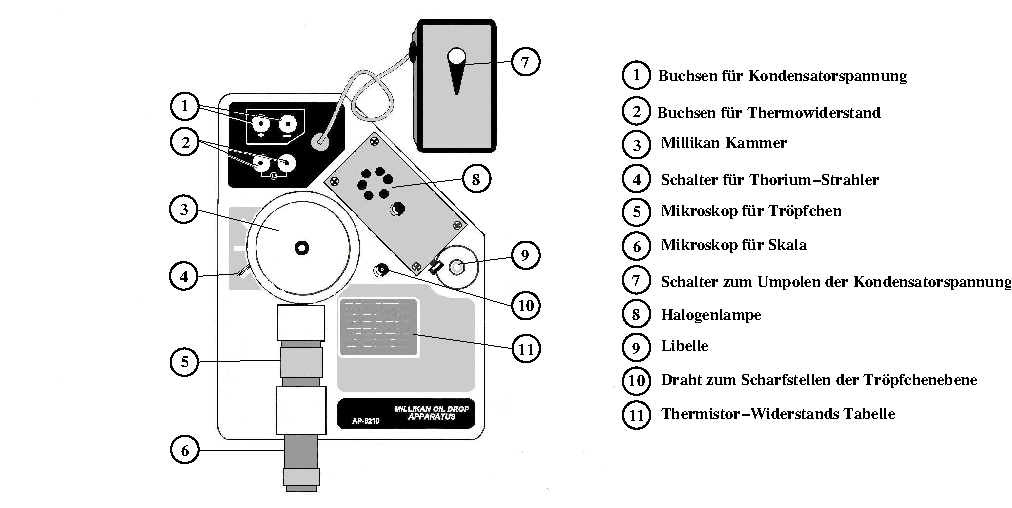
\includegraphics[width=1.0\textwidth]{figures/Abb2.pdf}
    \caption{Aufbau des Millikan-Öltröpfchenversuchs \cite{ap12}.}
    \label{fig:abb2}
\end{figure}

\subsection{Versuchsdurchführung}
Am Anfang muss sich die Aperatur in die Wagerechte befinden. Die Lage im Raum kann mit der Libelle $(9)$ kontrolliert werden.

Das Feld zwischen den Platten wird abgeschaltet. Danach wird eine hinreichende Anzahl an Öltröpfchen zwischen die Kondensatorplatten gesprüht. \\

Öltröpfchen mit einer Geschwindigkeit zwischen $v = 0.1 \, \unit{\milli\meter} \mathbin{/} \unit{\second}$ und $v = 0.01 \, \unit{\milli\meter} \mathbin{/} \unit{\second}$ eignen sich am besten zur Beobachtung.
Danach sollte geprüft werden, ob das beobachtete Tröpfchen geladen ist. Das Thorium-232 kann dazu verwendet werden, um die Ladung des Tröpfchens zu erhöhen. Währenddessen sollte $(7)$ auf " $OFF$ "${}$ stehen. \\

Die eigentliche Messung beginnt damit, dass das elektrische Feld mit $(7)$ eingeschaltet wird und die Zeit gemessen, die das Tröpfchen braucht, um eine bestimmte Strecke zurück zulegen.
Danach wird das Feld umgepolt $ (7) $ und die gleiche Strecke durchlaufen. Es wird erneut die Zeit gemessen. Für eine größere Messgenauigkeit kann dieser Prozess mehrfach wiederholt werden.
Im Anschluss wird die Geschwindigkeit $v_0$ gemessen. \\

Dieser Messprozess wird für vier weitere Tröpfchen wiederholt.\\

Im Anschluss wird die Messung für andere Kondensatorspannungen wiederholt. Die Spannung liegt dabei zwischen $150 \, \unit{\volt}$ und $250 \, \unit{\volt}$\\

Die Halogenlampe $(8)$ kann angeschaltet werden, damit die Öltröpfchen in der Kammer besser zu erkennen sind.
Ist die Lampe eingeschaltet erwärmt sie die Millikan Kammer $(3)$, deswegen muss die Temperatur regelmäßig.
